\documentclass[12pt]{article}
\pagestyle{plain}
\usepackage{pslatex}
\usepackage[usenames]{color}
\usepackage{graphicx}
\textwidth=16cm
\textheight=26.0cm
\topmargin 0.2in

\begin{document}
\setlength{\oddsidemargin}{-.3cm}
\setlength{\topmargin}{-2.cm}

\Large \begin{center}
Data structures of the wavelet program
\end{center} 

\large \begin{center}
Stefan Goedecker
\end{center} 
\normalsize \begin{center}
Institut f\"{u}r Physik \\
Universit\"{a}t Basel, Switzerland \\
\end{center} 

\noindent
The molecule is covered by a global grid of dimensions { \color{red} 0:n1, 0:n2, 0:n3}.
The values $n_1,n_2,n_3$ are not input values but are calculated by the program as described below.
The input parameter is the grid spacing { \color{red} hgrid}. 
The real space location of a grid point (i1,i2,i3) is (i1*hgrid, i2*hgrid, i3*hgrid). 
The molecule is shifted by the program such that it is covered by this grid. There 
are three types of grid points. 
In addition there are local grids for the individual orbitals whose dimension 
is denoted in the program by the variables { \color{red} nl1:nu1, nl2:nu2, nl3:nu3}.
The local grids are always inside the global grid. Both the single global grid as 
well as the various local grids consist of 
\begin{itemize}
\item grid points far from any atom that do not carry any basis function
\item grid points in the coarse region carry a scaling function 
\item grid points in the fine resolution that carry in addition 7 wavelets. 
\end{itemize}

The global grid points in the coarse region are all the grid points that satisfy 
the property that they are closer to some atom of type $ityp$ than 
{ \color{red} rcmult*radii\_cf(ityp,1)}.  The values 
of the array radii\_cf are read from the second line of the pseudopotential files.
The values radii\_cf(*,1) give the assymptotic decay length of the wavefunction, 
$1/\sqrt{2 \epsilon_{HOMO}}$.  The global grid points in the fine region are 
determined in the same way except that the distance 
criterion is { \color{red} rfmult*radii\_cf(ityp,2)}. 
radii\_cf(ityp,2) gives the radius where the 
pseudopotential of an atom of type ityp varies  strongly.
The factors rcmult and rfmult are read from the input file

The coarse and fine regions of the local grids are determined in the same way, except 
that in the above definitions not all the atoms are used but only the atoms belonging 
to the localization region of an orbital. So typically a localization region 
consists of a fine resolution region containing the few atoms forming the localization 
region and a much larger coarse resolution region. The determination of the localization 
region is at present based on the covalent radii of the atoms that 
are read from the second line of the pseudopotential files (third entry) and the 
parameter { \color{red} radlocmult} that is read from the input file. Putting 
radlocmult to a very large value will results in completely delocalized orbitals.
The array { \color{red} loregion} specifies which atom centered spheres contribute 
to the localization region of a certain orbital.
The various local grids are written into the files { \color{red} grid*.ascii} 
that can be visualized with V\_SIM. 

The picture below shows a global grid for a silicon cluster

\vspace{3cm}
\begin{figure}[ht]             % produce figure
\begin{center}
\setlength{\unitlength}{1cm}
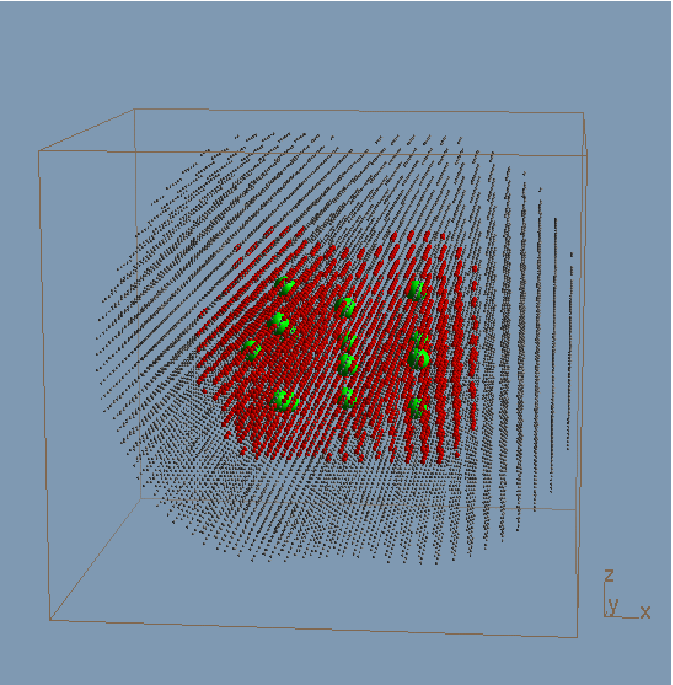
\includegraphics[width=0.5\textwidth]{figrid.pdf}
\caption{ \label{grid} Grid around a silicon cluster. Atoms are big green spheres, 
grid points in the fine resolution region are shown in red, coarse resolution grid points 
in black.}
\end{center}
\end{figure}

\pagebreak 

\noindent
Since not all grid points carry scaling functions and wavelets and since 
the coarse and fine resolution domains are irregular, the expansion 
coefficients of the wavefunctions are stored in compressed form. First the 
3-dim grid is mapped onto an 1-dim array of length (n1+1) * (n2+1) * (n3+1). Then grid points 
carrying no basis functions are eliminated by compressing the data as shown below.

\begin{figure}[ht]             % produce figure
\begin{center}
\setlength{\unitlength}{1cm}
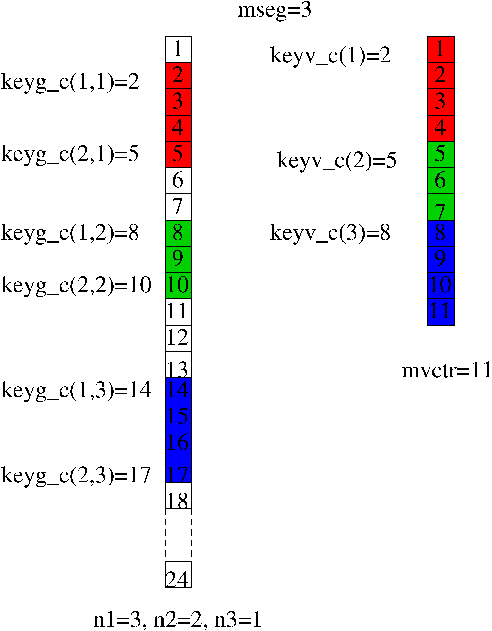
\includegraphics[width=0.5\textwidth]{compress.pdf}
\caption{ \label{compress} The data compression scheme. The subscripts \_c has to be replaced 
by \_f for the fine part.}
\end{center}
\end{figure}

\section{data structures in routines acting on a single orbital}
Since there are typically lines along the x-axis whose grid points all carry basis functions, 
the compression is based on segments. In the present implementation, a segment can not 
contain the grid point of more than onle line. {\color{red} mseg\_c} and 
{\color{red} mseg\_f} give the 
number of segments for the scaling functions and wavelets. The compression of the 
wavelets is similar except that each box holds 7 data items. A compressed wavefunction consists 
of two vectors {\color{red} psi\_c(mvctr\_c)} and {\color{red} psi\_f(7,mvctr\_f)}. 
{\color{red} keyg\_c(1,*)} and {\color{red} keyg\_f(1,*)}  give the starting points of the segments and
{\color{red} keyg\_c(2,*)} and {\color{red} keyg\_f(2,*)} give the end points of the segments in 
the vector of length (n1+1)*(n2+1)*(n3+1). {\color{red} keyv\_c(*)} gives the 
starting points in the compressed vector. A separate array for the end points is not 
necessary since there are no holes in the compressed data structure. 

A single projector has exacly the same data structure. The coarse and fine regions for 
one projectors are given by the condition that the distance of the grid point to 
the atom to which the projector belongs is less than  cpmult*radii\_cf(*,2) and less 
than fpmult*radii\_cf(*,2), where {\color{red} cpmult, fpmult} are read from the input file.


\section{data structures in routines acting on all orbitals}
The scaling function and wavelet expansion coefficients of all the orbitals are 
contained in the array {\color{red} psi}. The number of segments and the number of 
vector elements of all the orbitals is contained in the arrays {\color{red} nseg} and 
{\color{red} nvctr}. 
{\color{red} norb} is the number of real space orbitals which is equal to (half) 
of the number of electrons for a (non)-spinpolarized calculation.

\begin{verbatim}
do iorb=1,norb
   mseg_c=nseg(2*iorb-1)-nseg(2*iorb-2)   !number of coarse segments
   mseg_f=nseg(2*iorb  )-nseg(2*iorb-1)   !number of fine segments
   iseg_c=nseg(2*iorb-2)+1                !starting adress for coarse seg.
   iseg_f=nseg(2*iorb-1)+1                !starting adress for fine seg.
   mvctr_c= nvctr(2*iorb-1)-nvctr(2*iorb-2)    !# of coarse vector elem.
   mvctr_f=(nvctr(2*iorb  )-nvctr(2*iorb-1))/7 !# of fine vector elem./7
   ipsi_c=nvctr(2*iorb-2)+1            !starting address for coarse coef.
   ipsi_f=nvctr(2*iorb-1)+1            !starting address for fine coef.
   nl1=nbox_c(1,1,iorb) ; nu1=nbox_c(2,1,iorb)   ! local gridsize
   nl2=nbox_c(1,2,iorb) ; nu2=nbox_c(2,2,iorb)
   nl3=nbox_c(1,3,iorb) ; nu3=nbox_c(2,3,iorb)

!   call a routine that acts on a single orbital
   call singleorbital(n1,n2,n3,nl1,nu1,nl2,nu2,nl3,nu3,  &
              mseg_c,mvctr_c,keyg(1,iseg_c),keyv(iseg_c),   &
              mseg_f,mvctr_f,keyg(1,iseg_f),keyv(iseg_f),   &
              psi(ipsi_c),psi(ipsi_f),...............)
end do
\end{verbatim}

For the projectors there is not one individual decriptor array (keyg, keyv) for 
each projector, but only one descriptor array per atom (with a separable part)


\section{Miscalleneous}
The atom types are specified by their pseudopotential. 
The parameters for the different pseudopotentials are contained in the 
the psppar.* files.
The pseudopotential type follows in the input file after the 3 cartesian coordinates. 
For instance \newline
 0.  0. 0.  Si\_lda  \newline 
means that the atom at the origin is described by the pseudopotential 
file psppar.Si\_lda.

If the parameter { \color{red} calc\_inp\_wf } in the input file is set to true an 
input guess for the wavefunctions is calculated.
If  calc\_inp\_wf is false initial wavefunctions are assumed to be in the 
wavefunction files and they are only read in from these files. If the wavefunctions 
in the wavefunction files were calculated with a different set of parameters (eg. 
different hgrid or rcmult) the readwave subroutine can do the necessary 
transformations. 

\end{document}
